% =====================================================================
% Artigo final - Trabalho Computacional de Pesquisa Operacional (UFMG)
% Compilar no Overleaf com pdfLaTeX + BibTeX (arquivo principal: artigo.tex)
%
% Trechos em vermelho marcados com \afazer{...} devem ser escritos ou
% revisados pelo grupo antes da entrega (procure por "afazer").
%
% Números e tabelas vêm de tabelas/*.tex, gerados por gera_tabelas_latex.py
% a partir dos resultados do código (não edite esses arquivos à mão).
% =====================================================================
\documentclass[11pt,a4paper]{article}

\usepackage[utf8]{inputenc}
\usepackage[T1]{fontenc}
\usepackage[brazil]{babel}
\usepackage{lmodern}
\usepackage[a4paper,margin=2.5cm]{geometry}
\usepackage{amsmath,amssymb}
\usepackage{graphicx}
\usepackage{booktabs}
\usepackage{array}
\usepackage{verbatim}
\usepackage{xcolor}
\usepackage[font=small,labelfont=bf]{caption}
\usepackage[round,authoryear]{natbib}
\usepackage[hidelinks]{hyperref}

\graphicspath{{figuras/}}
% Gerado por gera_tabelas_latex.py -- não editar à mão
\newcommand{\lambdaCentral}{0{,}435}
\newcommand{\lambdaCalibrado}{0{,}435}
\newcommand{\lambdaGargalo}{0{,}43}
\newcommand{\lambdaMinLinha}{0{,}22}
\newcommand{\lambdaMaxLinha}{0{,}73}
\newcommand{\Zotimo}{276.041{,}95}
\newcommand{\custoTotal}{264.416{,}95}
\newcommand{\esperaPash}{465}
\newcommand{\esperaMin}{0{,}32}
\newcommand{\demandaTotal}{86.310}
\newcommand{\viagensTotal}{712}
\newcommand{\viagensGTFS}{664}
\newcommand{\variacaoViagens}{7{,}2}
\newcommand{\custoGTFS}{242.902{,}32}
\newcommand{\variacaoCusto}{8{,}9}
\newcommand{\esperaMinGTFS}{35{,}0}
\newcommand{\ZGTFS}{1.500.427}
\newcommand{\perdidosGTFS}{4.245}
\newcommand{\pctPerdidosGTFS}{4{,}92}
\newcommand{\perdidosOtimo}{392}
\newcommand{\pctPerdidosOtimo}{0{,}45}
\newcommand{\custoPerdaGTFS}{242.902}
\newcommand{\custoPerdaOtimo}{262.994}
\newcommand{\embViagemCentral}{130{,}0}
\newcommand{\embViagemUm}{171{,}2}
\newcommand{\esperaLambdaZero}{0{,}05}
\newcommand{\esperaLambdaUm}{8{,}36}
\newcommand{\frotaNecZero}{79}
\newcommand{\frotaNecUm}{102}
\newcommand{\frotaNecCentral}{99}
\newcommand{\precoLambdaUm}{13.255}
\newcommand{\frotaMax}{97}
\newcommand{\frotaMOVE}{457}
\newcommand{\capCorredor}{64}
\newcommand{\esperaFnoventa}{1{,}59}
\newcommand{\esperaMaisDezArt}{0{,}16}
\newcommand{\esperaPadron}{0{,}16}
\newcommand{\custoPadron}{256.980}
\newcommand{\custoMaisDezArt}{265.095}
\newcommand{\viagensPadron}{107}
\newcommand{\equilibrioPadron}{899}
\newcommand{\equilibrioMaisDezArt}{510}
\newcommand{\equilibrioPadronIgual}{340}
\newcommand{\viagensPadronIgual}{9}
\newcommand{\equilibrioMaisDezArtUm}{6.991}
\newcommand{\esperaBase}{0{,}32}
\newcommand{\custoBase}{264.417}
\newcommand{\esperaBaseUm}{8{,}36}
\newcommand{\esperaCorredorUm}{8{,}23}
\newcommand{\esperaMaisDezArtUm}{6{,}89}
\newcommand{\Zrelax}{257.280{,}40}
\newcommand{\gapInt}{6{,}80}
\newcommand{\gapFinal}{0{,}0031}
\newcommand{\cortesGomory}{26}
\newcommand{\cortesMIR}{64}
\newcommand{\nosExplorados}{1}
\newcommand{\iteracoesSimplex}{101}
\newcommand{\tempoSolucao}{0{,}11}
\newcommand{\presolveLinhas}{138}
\newcommand{\presolveColunas}{204}
\newcommand{\horaPrecoMax}{7h}
\newcommand{\precoSombraMax}{6.042{,}40}
\newcommand{\deltaPLIMMax}{2.971{,}26}
\newcommand{\faixasReotimizadas}{24}
\newcommand{\faixasGanhoPLIM}{1}
\newcommand{\regimeFolga}{66}
\newcommand{\regimeLimite}{14}
\newcommand{\regimeFila}{2}
\newcommand{\regimeSobra}{23}
\newcommand{\regimeSemDemanda}{15}
\newcommand{\nPares}{120}
\newcommand{\custoMarginalPareto}{21{,}82}
\newcommand{\alfaUm}{1}
\newcommand{\alfaDois}{25}
\newcommand{\margemTerminal}{15}
\newcommand{\nVarInt}{240}
\newcommand{\nVarCont}{120}
\newcommand{\versaoGurobi}{13.0.3}
\newcommand{\embarquesEstacoes}{99.360}
\newcommand{\demandaSup}{113.645}
\newcommand{\demandaInf}{65.266}
\newcommand{\tempoLimite}{60}
\newcommand{\nRestr}{393}


\newcommand{\afazer}[1]{{\color{red}\textbf{[A FAZER:} #1\textbf{]}}}
\newcommand{\R}{\mathbb{R}}
% tabelas largas: reduz para caber na largura do texto
\newcommand{\tabela}[1]{\resizebox{\ifdim\width>\textwidth\textwidth\else\width\fi}{!}{\input{#1}}}

\title{Otimização de Frequências e Tipos de Veículo das Linhas Troncais do MOVE\\no Corredor Antônio Carlos com Programação Linear Inteira Mista}
\author{\afazer{Nome 1} \and \afazer{Nome 2} \and \afazer{Nome 3}\\[4pt]
\small Pesquisa Operacional -- Departamento de Engenharia Elétrica -- UFMG}
\date{Novembro de 2026}

\begin{document}
\maketitle

\begin{abstract}
Este trabalho define, para as cinco linhas troncais do MOVE no Corredor Antônio
Carlos (Belo Horizonte), quantas viagens de cada tipo de veículo devem partir em
cada hora de um dia útil. O problema é formulado como um Programa Linear Inteiro
Misto (PLIM) que minimiza o custo operacional e a espera excedente dos
passageiros, sujeito à frota disponível -- contabilizada ao longo de todo o
ciclo de cada viagem --, à capacidade do corredor, a um padrão mínimo de serviço
e a uma fila de passageiros entre faixas horárias. A oferta e a frota atuais vêm
do GTFS da BHTRANS e a demanda, dos embarques registrados nos relatórios mensais
da BHTRANS. Como o rateio dos embarques das estações entre as linhas é incerto,
a demanda é delimitada por um intervalo e calibrada de modo que a grade atual
tenha ocupação média de 100\% ($\lambda=\lambdaCentral$). Nesse cenário, a
solução ótima oferece mais serviço que a grade atual por um custo
\variacaoCusto\% maior, com espera excedente de \esperaMin{} minuto por
passageiro. A escassez de frota no pico da manhã só aparece a partir de
$\lambda\approx\lambdaGargalo$; no limite inferior da demanda, a frota atual
sobra. A fronteira de Pareto, os cenários de frota e a análise de dualidade
completam a análise.
\end{abstract}

% =====================================================================
\section{Introdução}
% =====================================================================

O transporte coletivo por ônibus é o principal modo de deslocamento de grande
parte da população de Belo Horizonte. O MOVE, sistema de BRT (\emph{Bus Rapid
Transit}) da cidade, opera em corredores exclusivos, entre eles o da Av.~Antônio
Carlos / Av.~Pedro~I, que liga as regiões de Venda Nova e da Pampulha ao centro.
Nas estações desse corredor são registrados, em média, \embarquesEstacoes{}
embarques por dia útil \citep{bhtrans2026}.

Definir a frequência de cada linha -- quantas viagens por hora ela realiza -- é
uma das etapas centrais do planejamento operacional \citep{ceder2016}.
Frequência baixa deixa passageiros nos pontos e provoca superlotação; frequência
alta aumenta o custo e exige mais veículos, um recurso limitado e compartilhado
entre linhas e horários. A decisão envolve, portanto, um \emph{trade-off} entre
nível de serviço e custo, acoplado pela frota.

\afazer{Revisar e completar: relevância do problema para BH, contexto do MOVE e
motivação do grupo.}

Este artigo formula o problema como um PLIM e o resolve de forma exata com o
Gurobi. As contribuições são: (i) uma restrição de frota acumulada, que
contabiliza os ônibus que partiram em faixas anteriores e ainda não retornaram;
(ii) o tipo de veículo como variável de decisão; (iii) uma fila de passageiros
entre faixas horárias; (iv) uma instância construída com dados abertos reais,
com a demanda calibrada pela grade atual e analisada em todo o intervalo
compatível com os dados; e (v) a fronteira de Pareto custo $\times$ nível de
serviço e uma análise de dualidade.

O artigo está organizado assim: a Seção~\ref{sec:revisao} revisa a literatura; a
Seção~\ref{sec:modelo} descreve o problema, o modelo e os dados; a
Seção~\ref{sec:algoritmo}, o método de solução; a Seção~\ref{sec:resultados}
apresenta os resultados; e a Seção~\ref{sec:conclusao} conclui.

% =====================================================================
\section{Revisão da literatura}\label{sec:revisao}
% =====================================================================

\afazer{Esta seção é avaliada como pesquisa bibliográfica do grupo. O professor
espera um parágrafo por referência, discutindo de forma crítica o modelo, a
ferramenta de solução e os resultados de cada trabalho. Meta: 6 a 8 trabalhos.
Os dois parágrafos abaixo são pontos de partida -- confiram nas fontes originais
e reescrevam com as palavras do grupo.}

\citet{ceder2016} sistematiza os métodos de definição de frequências usados na
prática, baseados em dados de carregamento (passageiros no ponto de carga
máxima) e em padrões de frequência mínima. Esses métodos dimensionam cada linha
separadamente; a frota disponível não entra como restrição conjunta entre
linhas, que é o acoplamento tratado neste trabalho.
\afazer{Conferir no livro e aprofundar.}

\citet{arbex2015} tratam conjuntamente o projeto da rede e a definição de
frequências como um problema multiobjetivo, minimizando o custo dos passageiros
e o custo do operador, e o resolvem com um algoritmo genético de objetivos
alternados. A abordagem lida com um problema maior (inclui o traçado das
linhas), mas, por ser heurística, não garante otimalidade; aqui, com as linhas
fixas, o problema é linear e é resolvido de forma exata.
\afazer{Conferir no artigo: instâncias usadas, resultados obtidos.}

\afazer{Acrescentar 4 a 6 trabalhos. Sugestões de busca (Google Scholar,
Periódicos CAPES): ``frequency setting problem'', ``transit frequency
optimization'', ``mixed fleet'' / ``vehicle type frequency setting'', ``line
planning'' (ver \citet{schmidt2024}), revisões sobre planejamento de ônibus e
trabalhos brasileiros sobre BRT.}

% =====================================================================
\section{Descrição do problema e modelagem}\label{sec:modelo}
% =====================================================================

\subsection{Problema}

Considera-se o conjunto $L$ das linhas troncais do MOVE no Corredor Antônio
Carlos (51, 52, 63, 64 e 67), o conjunto $T=\{0,\dots,23\}$ das faixas horárias
de um dia útil e o conjunto $K$ dos tipos de veículo (articulado e Padron). As
linhas são circulares: cada viagem parte de uma estação de integração, percorre
o corredor até o centro e retorna. Deseja-se decidir quantas viagens de cada
tipo cada linha realiza em cada faixa, minimizando um compromisso entre o custo
operacional e a espera excedente dos passageiros. As decisões estão acopladas:
os ônibus de cada tipo são compartilhados entre as linhas e permanecem ocupados
por mais de uma faixa; as linhas disputam a capacidade do corredor; e quem não
embarca numa faixa continua esperando na seguinte.

\subsection{Modelo matemático}

\paragraph{Parâmetros.}
$c_{ltk}=D_{lt}\cdot\text{(custo/km)}_k$ é o custo de uma viagem; $D_{lt}$ é a
extensão da viagem (ida e volta); $n_{lt}$ é o tempo de ciclo (h); $C_k$ é a
capacidade e $F_k$ a frota disponível do tipo $k$; $d_{lt}$ é a demanda, em
embarques por hora atribuídos à linha (Seção~\ref{sec:dados}); $\bar{P}$ é a
capacidade do corredor (partidas/h); $f^{\min}_{lt}$ e $f^{\max}_{lt}$ são
limites de frequência; e $\alpha_1,\alpha_2$ são os pesos da função objetivo. A
Tabela~\ref{tab:fontes} lista os valores e a origem de cada parâmetro.

\paragraph{Variáveis.}
$f_{ltk}\in\mathbb{Z}_{\ge 0}$ é o número de partidas do tipo $k$ da linha $l$ na
faixa $t$; $w_{lt}\in\R_{\ge 0}$ é o número de passageiros que terminam a faixa
$t$ ainda esperando.

\paragraph{Formulação.}
\begin{align}
\min\; Z = {} & \alpha_1 \sum_{l,t,k} c_{ltk}\, f_{ltk} \;+\; \alpha_2 \sum_{l,t} w_{lt} \label{eq:fo}\\
\text{s.a.}\quad
& \sum_{l\in L}\sum_{s\in T} \omega\!\left(t-s,\, n_{ls}\right) f_{lsk} \;\le\; F_k
  && \forall\, t\in T,\ k\in K \label{eq:frota}\\
& \sum_{k\in K} C_k\, f_{ltk} + w_{lt} \;\ge\; d_{lt} + w_{l,t-1}
  && \forall\, l\in L,\ t\in T \label{eq:demanda}\\
& \sum_{l\in L}\sum_{k\in K} f_{ltk} \;\le\; \bar{P}
  && \forall\, t\in T \label{eq:corredor}\\
& f^{\min}_{lt} \;\le\; \sum_{k\in K} f_{ltk} \;\le\; f^{\max}_{lt}
  && \forall\, l\in L,\ t\in T \label{eq:padrao}\\
& f_{ltk}\in\mathbb{Z}_{\ge0},\quad w_{lt}\ge 0,\quad w_{l,-1}=0. \notag
\end{align}

A restrição~\eqref{eq:demanda} faz com que quem não embarca na faixa $t$ entre na
demanda de $t+1$; assim, $\sum w_{lt}$ é a espera excedente em
passageiro-hora, e $\alpha_2$ é o valor (R\$) atribuído a cada passageiro-hora.
Para comparar instâncias, usa-se a espera excedente média por passageiro,
$60\sum w_{lt}/\sum d_{lt}$ (minutos). Como variante, o modo ``perda'' remove o
termo $w_{l,t-1}$ (o passageiro não atendido desiste) e mede a porcentagem de
passageiros perdidos. A restrição~\eqref{eq:corredor} limita as partidas por
hora no corredor e~\eqref{eq:padrao} impõe um intervalo máximo entre ônibus
(padrão de serviço).

Os índices de tempo de~\eqref{eq:frota} são cíclicos (os ônibus que partem às
23h ainda ocupam a frota à 0h), enquanto a fila começa vazia ($w_{l,-1}=0$).
A assimetria é deliberada: o dia útil começa sem passageiros acumulados, e a
madrugada tem demanda e frota muito pequenas.

\paragraph{Restrição de frota acumulada.}
Um ônibus que parte num instante $u$ da faixa $s$, com $u$ uniforme em $[0,1)$,
permanece em operação no intervalo $[u,\,u+n]$. A fração média da faixa $s+j$
que ele ocupa é
\begin{equation}
\omega(j,n) \;=\; \int_0^1 \bigl|\,[u,\,u+n]\cap[j,\,j+1]\,\bigr|\; du .
\end{equation}
A frota em operação na faixa $t$ soma as partidas de $t$ e as de faixas
anteriores que ainda não retornaram. Como $\sum_j \omega(j,n)=n$, para
frequência constante~\eqref{eq:frota} se reduz à relação clássica
$\text{frota}=\text{frequência}\times\text{ciclo}$ \citep{ceder2016}; a diferença
aparece nas transições de demanda, como o início dos picos. Os pesos $\omega$ são
calculados previamente, e a restrição permanece linear.

\paragraph{Estrutura e porte.}
Sem as restrições~\eqref{eq:frota} e~\eqref{eq:corredor} e sem a fila, cada par
$(l,t)$ seria independente e a solução trivial seria $f=\lceil d/C\rceil$. O
problema é combinatório porque a frota acumulada acopla linhas e faixas
vizinhas, o corredor acopla as linhas, a fila acopla as faixas e os tipos de
veículo competem pela mesma demanda. A instância tem \nVarInt{} variáveis
inteiras, \nVarCont{} contínuas e \nRestr{} restrições.

\begin{table}[htbp]
\centering
\caption{Parâmetros, valores e origem (GTFS e BHTRANS: dados oficiais; hipótese: valor adotado pelo grupo).}
\label{tab:fontes}
\small
\tabela{tabelas/parametros_fontes.tex}
\end{table}

\subsection{Dados e instância}\label{sec:dados}

\paragraph{Oferta e frota (GTFS e BHTRANS).}
Tempos de viagem, extensões e calendário foram extraídos do GTFS da BHTRANS
\citep{gtfsbhtrans}, considerando as viagens de dia útil de todas as variantes
regulares. A extensão foi calculada a partir da geometria de cada itinerário,
projetada em SIRGAS~2000 / UTM~23S. Por linha e faixa, extensão e tempo de ciclo
são médias ponderadas pelas viagens de cada variante, com margem de
\margemTerminal\% no terminal. A frota disponível é a frota em operação exigida
pela grade atual (\viagensGTFS{} viagens por dia), calculada com a mesma
regra~\eqref{eq:frota}: $F=\frotaMax$ veículos. Como verificação, a BHTRANS
informa uma frota cadastrada de \frotaMOVE{} veículos no BRT MOVE, somando todos
os corredores e incluindo a reserva técnica \citep{bhtrans2026}; o relatório não
detalha a frota por linha. Assim, $F$ representa os veículos em operação,
sem a reserva. A capacidade do corredor é o maior número de partidas por hora
programado hoje ($\bar{P}=\capCorredor$). Como $F$ e $\bar{P}$ vêm da própria
grade (e da margem de terminal adotada), eles medem a operação atual, e não a
capacidade máxima do sistema.

\begin{table}[htbp]
\centering
\caption{Parâmetros por linha (GTFS) e demanda na instância calibrada.}
\label{tab:parametros}
\small
\tabela{tabelas/parametros_linhas.tex}
\end{table}

\paragraph{Demanda (BHTRANS).}
Os relatórios mensais da BHTRANS publicam, para o corredor, os passageiros
registrados por linha e por estação \citep{bhtrans2026}; usou-se a média de dias
úteis de março a agosto de 2026. Os dados são \emph{embarques}, e não carga
medida no trecho crítico; considera-se, de forma conservadora, que cada
embarque ocupa o veículo no trecho de maior lotação (um fator de conversão que,
na calibração abaixo, não é identificável separadamente de $\lambda$). No MOVE,
quem embarca numa estação passa pela catraca da estação e é registrado nela, e
não na linha. A demanda de cada linha é, então, o registro no próprio ônibus
mais uma parcela dos \embarquesEstacoes{} embarques diários nas estações,
rateada pelas viagens programadas. Como outras linhas também usam as estações,
há dois limites (Tabela~\ref{tab:demanda}): o inferior (\demandaInf{} embarques
por dia) rateia os embarques entre todas as linhas listadas no corredor e o
superior (\demandaSup{}), só entre as cinco do modelo. A instância é
parametrizada por $\lambda\in[0,1]$: demanda $=$ inferior $+\,\lambda\,($superior
$-$ inferior$)$. A demanda diária é distribuída pelas horas proporcionalmente às
viagens programadas.

\begin{table}[htbp]
\centering
\caption{Demanda diária por linha (embarques por dia útil) e $\lambda$ em que a grade atual de cada linha satura.}
\label{tab:demanda}
\small
\tabela{tabelas/demanda_bhtrans.tex}
\end{table}

\paragraph{Calibração de $\lambda$.}
Adota-se como cenário central o $\lambda$ em que a capacidade total da grade
atual (viagens programadas $\times$ 130 lugares) iguala a demanda total, isto é,
em que a grade que de fato opera tem ocupação média de 100\%:
$\lambda=\lambdaCentral$. A justificativa é que a operadora não programaria uma
grade estruturalmente insuficiente, nem com grande sobra. Todos os resultados
também são apresentados para o intervalo completo de $\lambda$
(Seção~\ref{sec:lambda}).

\paragraph{Limitações: circularidade e rateio.}
Como o rateio e o perfil horário seguem a grade atual, cada viagem programada de
uma linha recebe o mesmo número de embarques. Duas consequências precisam ser
explícitas. Primeiro, a diferença de demanda \emph{entre} as linhas vem de quanto
cada uma registra a bordo: as linhas 51, 64 e 67 operam também fora das estações
e registram milhares de embarques no ônibus, enquanto as linhas 52 e 63
praticamente não registram. Por isso a grade de cada linha satura em valores de
$\lambda$ muito diferentes (de \lambdaMinLinha{} a \lambdaMaxLinha{},
Tabela~\ref{tab:demanda}). Segundo, a comparação com a grade atual por linha
recupera, em parte, essa regra de construção da demanda. Testa-se a
circularidade com um perfil horário típico, independente da grade
(Seção~\ref{sec:robustez}). A demanda também não inclui os passageiros que
chegam por linhas alimentadoras e se transferem nas estações de integração.

% =====================================================================
\section{Descrição do algoritmo}\label{sec:algoritmo}
% =====================================================================

O modelo foi implementado em Python, com a interface \texttt{gurobipy}, e
resolvido pelo Gurobi Optimizer \versaoGurobi{} \citep{gurobi2026}. Como há
variáveis inteiras, o Gurobi aplica \emph{branch-and-cut}, que combina
\emph{branch-and-bound} com planos de corte \citep{arenales2007, hillier2013}:
\begin{enumerate}
\item \textbf{Pré-processamento:} simplifica o modelo; aqui, reduziu-o a
\presolveLinhas{} restrições e \presolveColunas{} variáveis.
\item \textbf{Relaxação linear} pelo método simplex, que fornece um limite
inferior para o ótimo (R\$~\Zrelax{}).
\item \textbf{Planos de corte:} desigualdades válidas que eliminam soluções
fracionárias; o log registra \cortesGomory{} cortes de Gomory e \cortesMIR{}
cortes MIR.
\item \textbf{Heurísticas primais} para encontrar soluções inteiras (limite
superior).
\item \textbf{Ramificação} sobre variáveis fracionárias, se necessário.
\item \textbf{Parada} quando o gap relativo entre os limites fica abaixo de
0{,}01\%.
\end{enumerate}
Na instância central, a solução ótima foi encontrada no nó raiz
(\nosExplorados{} nó, \iteracoesSimplex{} iterações do simplex,
\tempoSolucao{}~s), com gap final de \gapFinal\%. Os cortes fecharam a distância
de \gapInt\% entre a relaxação linear e o ótimo inteiro (gap de integralidade).
Nas análises mais pesadas (cenários com demanda alta), adotou-se um tempo limite
de \tempoLimite{}~s por resolução; os poucos casos que o atingiram são
reportados com o gap alcançado. O Apêndice~\ref{ap:log} reproduz o log.

\paragraph{Fronteira de Pareto.}
A soma ponderada~\eqref{eq:fo} só encontra soluções suportadas da fronteira.
Para obtê-la de forma completa usou-se o método $\varepsilon$-restrição: minimizar
o custo operacional sujeito a $\sum w_{lt}\le\varepsilon$, variando $\varepsilon$
entre a menor espera possível (obtida lexicograficamente) e uma espera média de
18 minutos por passageiro.

\paragraph{Dualidade e pós-otimização.}
Um PLIM não possui variáveis duais. Resolveu-se, então, a relaxação linear e
extraíram-se os preços-sombra das restrições de frota, corredor e atendimento,
as folgas e os intervalos do lado direito em que cada preço-sombra é válido
\citep{arenales2007}. Para validá-los no problema inteiro, o PLIM foi
re-otimizado com uma unidade a mais no lado direito de cada restrição de frota e
de corredor, em todas as faixas.

\paragraph{Implementação.}
Os parâmetros ficam em \texttt{config.py}; o modelo, em \texttt{modelo.py}; a
extração de dados em \texttt{extracao\_dados\_gtfs.py} e
\texttt{demanda\_pbh.py}; e cada análise num script próprio. O arquivo
\texttt{executar\_tudo.py} reproduz todos os resultados deste artigo.

% =====================================================================
\section{Resultados e análise}\label{sec:resultados}
% =====================================================================

\subsection{Solução da instância calibrada}

Com $\lambda=\lambdaCentral$ (\demandaTotal{} embarques por dia),
$F=\frotaMax$ articulados e $\alpha_2=$ R\$~\alfaDois{} por passageiro-hora, a
solução ótima tem $Z=$ R\$~\Zotimo{}, custo operacional de R\$~\custoTotal{},
\viagensTotal{} viagens e espera excedente de \esperaPash{} passageiro-hora
(\esperaMin{} minuto por passageiro) -- Tabela~\ref{tab:resultados}. A frota
fica no limite apenas às \horaPrecoMax{}, quando os ônibus que partiram no
início do pico ainda estão em circulação (Figura~\ref{fig:frota}).

\begin{table}[htbp]
\centering
\caption{Solução ótima por linha na instância calibrada (valores diários).}
\label{tab:resultados}
\small
\tabela{tabelas/resultados_linhas.tex}
\end{table}

\begin{figure}[htbp]
\centering
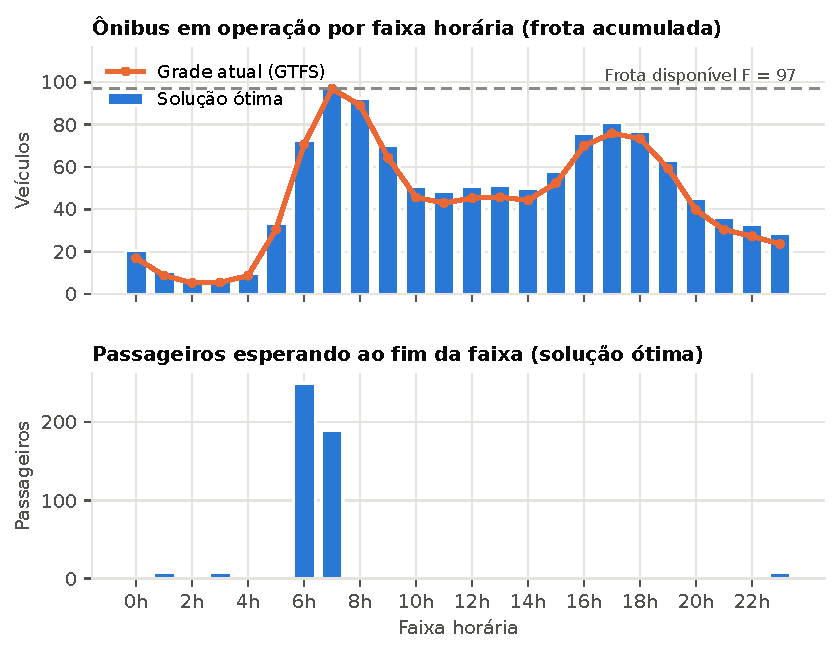
\includegraphics[width=0.85\textwidth]{frota_deficit_por_hora.pdf}
\caption{Ônibus em operação (solução ótima e grade atual) e passageiros esperando ao fim de cada faixa.}
\label{fig:frota}
\end{figure}

\subsection{Comparação com a grade atual}

A grade atual do GTFS foi avaliada com as mesmas regras do modelo e comparada à
solução ótima \emph{no mesmo modo} de tratamento dos não atendidos
(Tabela~\ref{tab:comparacao}). No modo fila, a grade atual custa
R\$~\custoGTFS{} por dia e gera espera média de \esperaMinGTFS{} minutos por
passageiro, porque a fila se acumula nas linhas cuja grade é insuficiente; a
solução ótima reduz a espera para \esperaMin{} minuto com custo
\variacaoCusto\% maior. No modo perda, a grade perderia \pctPerdidosGTFS\% dos
passageiros, contra \pctPerdidosOtimo\% da solução ótima. O resultado, portanto,
não é uma economia: é \emph{mais serviço por mais custo}, com a mesma frota e o
mesmo limite de corredor.

\begin{table}[htbp]
\centering
\caption{Grade atual (GTFS) $\times$ solução ótima, no mesmo modo de tratamento dos não atendidos.}
\label{tab:comparacao}
\small
\tabela{tabelas/validacao_comparacao.tex}
\end{table}

A Tabela~\ref{tab:validacao} detalha o modo perda por linha. O número de viagens
ótimo de cada linha fica próximo de $\sum_t\lceil d_{lt}/C\rceil$, o mínimo para
atender cada faixa isoladamente: o total por linha é determinado sobretudo pela
regra de construção da demanda. A ``redistribuição'' -- menos viagens nas linhas
52 e 63, mais nas linhas 51, 64 e 67 -- decorre, em grande parte, do rateio dos
embarques (Seção~\ref{sec:dados}), e a perda da grade atual por linha é, por
construção, o excesso de embarques por viagem sobre a capacidade. Essa parte da
comparação não é uma validação independente. O valor agregado do modelo está na
\emph{distribuição horária} das viagens e no \emph{acoplamento pela frota}: decidir
em que horas acrescentar viagens (Figuras~\ref{fig:partidas} e~\ref{fig:linhas})
sem ultrapassar a frota nas horas de pico.

\begin{table}[htbp]
\centering
\caption{Grade atual $\times$ solução ótima por linha (modo perda).}
\label{tab:validacao}
\small
\tabela{tabelas/validacao_linhas.tex}
\end{table}

\begin{figure}[htbp]
\centering
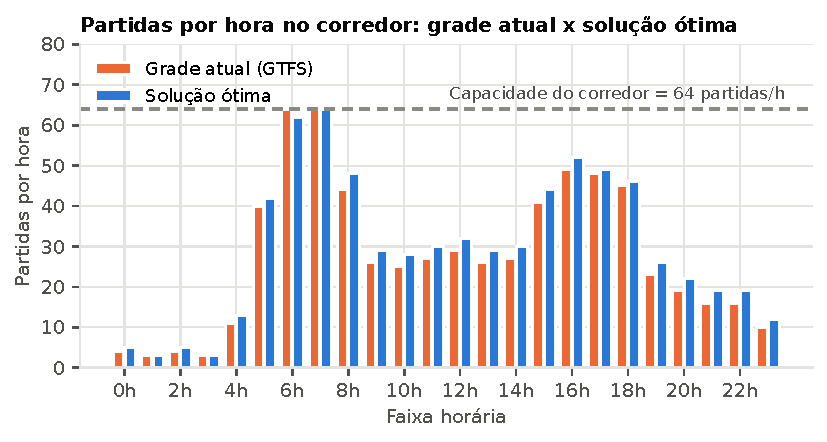
\includegraphics[width=0.85\textwidth]{validacao_partidas.pdf}
\caption{Partidas por hora no corredor: grade atual e solução ótima.}
\label{fig:partidas}
\end{figure}

\begin{figure}[htbp]
\centering
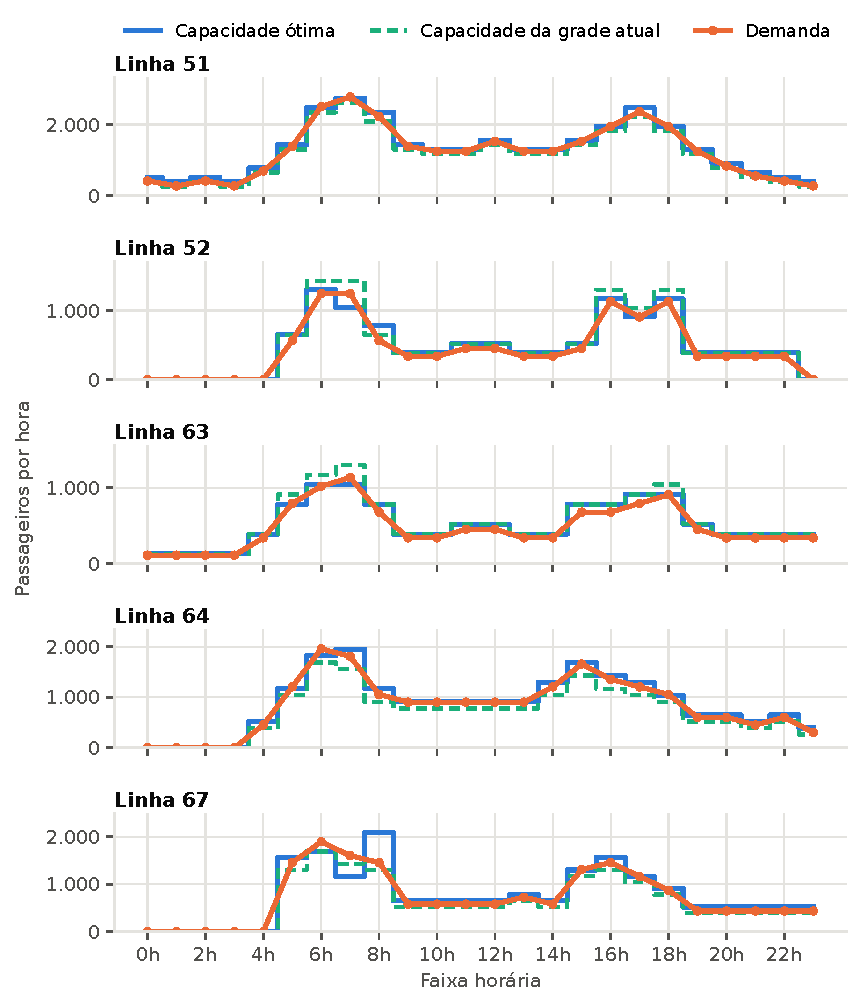
\includegraphics[width=0.85\textwidth]{demanda_capacidade_linhas.pdf}
\caption{Demanda, capacidade ótima e capacidade da grade atual por linha e faixa horária.}
\label{fig:linhas}
\end{figure}

\subsection{Resultados por nível de demanda}\label{sec:lambda}

A Tabela~\ref{tab:lambda} e a Figura~\ref{fig:lambda} repetem a otimização em
todo o intervalo de demanda. No limite inferior ($\lambda=0$), seriam
necessários apenas \frotaNecZero{} veículos, a espera é de
\esperaLambdaZero{} minuto e o preço-sombra da frota é nulo: não há escassez. O
preço-sombra passa a ser positivo a partir de $\lambda\approx\lambdaGargalo$, e
só a partir daí a frota é o gargalo. No limite superior, seriam necessários
\frotaNecUm{} veículos e a espera chega a \esperaLambdaUm{} minutos por
passageiro. A frota necessária não cresce de forma estritamente monotônica com
$\lambda$: quando o corredor passa a limitar as partidas nas horas de pico
(coluna ``faixas com corredor no limite''), parte da espera torna-se inevitável e
a frota adicional deixa de ajudar. Os valores numéricos devem, portanto, ser
lidos condicionados a $\lambda$; a conclusão de que a frota é o gargalo do pico
da manhã vale para $\lambda\gtrsim\lambdaGargalo$.

\begin{table}[htbp]
\centering
\caption{Resultados por nível de demanda ($\lambda=0$: limite inferior; $\lambda=1$: superior).}
\label{tab:lambda}
\small
\tabela{tabelas/demanda_lambda.tex}
\end{table}

\begin{figure}[htbp]
\centering
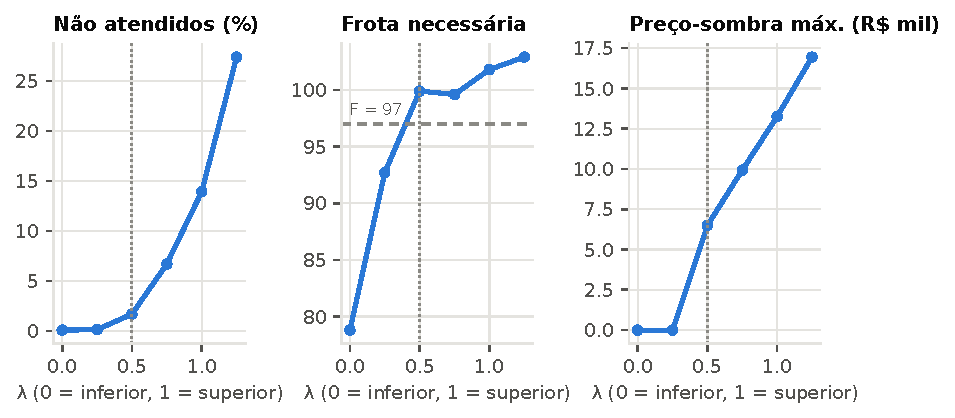
\includegraphics[width=0.9\textwidth]{demanda_lambda.pdf}
\caption{Espera média, frota necessária e maior preço-sombra da frota em função de $\lambda$ (linha pontilhada: instância calibrada).}
\label{fig:lambda}
\end{figure}

\subsection{Cenários de frota e infraestrutura}

Nos cenários da Tabela~\ref{tab:cenarios}, resolvidos na instância calibrada e
no limite superior de demanda, o modelo \emph{decide} o tipo de veículo de cada
viagem; o cenário só altera o que está disponível. Com 90 articulados (valor da
proposta inicial), a espera sobe para \esperaFnoventa{} minuto por passageiro.
Com 15 ônibus Padron a mais, a espera cai para \esperaPadron{} e o custo
operacional também cai, porque os Padron, mais baratos por quilômetro, assumem
\viagensPadron{} viagens. Essa conclusão, porém, depende de duas hipóteses: (i) o
custo operacional não inclui aquisição nem tripulação dos veículos extras; e
(ii) o custo por quilômetro do Padron é hipotético. Por isso a tabela reporta o
custo diário de equilíbrio por veículo extra -- o maior custo fixo que ainda
faria o cenário compensar em $Z$ -- e a sensibilidade ao custo/km do Padron. Com
custo/km igual ao do articulado, os 15 Padron compensam até
R\$~\equilibrioPadronIgual{} por veículo e por dia, contra
R\$~\equilibrioMaisDezArt{} de 10 articulados extras, de capacidade equivalente:
por veículo, o articulado rende mais, e a vantagem do Padron vem do custo/km
menor. No limite superior, 10 articulados extras reduzem a espera de
\esperaBaseUm{} para \esperaMaisDezArtUm{} minutos, enquanto ampliar o corredor
em 20\% a reduz apenas para \esperaCorredorUm{}: também com demanda alta, o
gargalo principal é a frota.

\begin{table}[htbp]
\centering
\caption{Cenários de frota e infraestrutura. ``Padron'': viagens feitas com Padron; ``Equilíbrio'': maior custo fixo diário por veículo acrescido que ainda reduz $Z$. $^\dagger$Tempo limite atingido (gap $\le 0{,}1\%$).}
\label{tab:cenarios}
\small
\tabela{tabelas/cenarios.tex}
\end{table}

\begin{figure}[htbp]
\centering
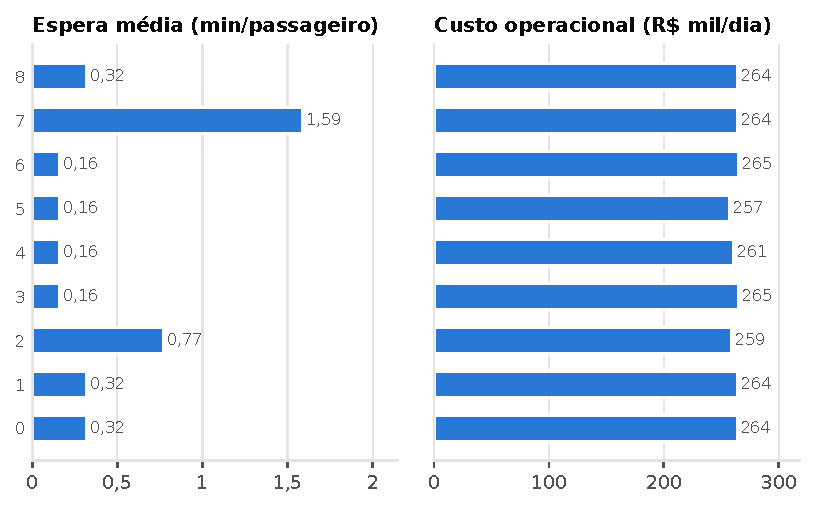
\includegraphics[width=0.9\textwidth]{cenarios.pdf}
\caption{Espera média e custo operacional por cenário (instância calibrada).}
\label{fig:cenarios}
\end{figure}

\subsection{Fronteira de Pareto e escolha de $\alpha_2$}

A Figura~\ref{fig:pareto} mostra a fronteira custo $\times$ espera obtida pelo
método $\varepsilon$-restrição e as soluções da soma ponderada para vários
valores de $\alpha_2$ (Tabela~\ref{tab:sensibilidade}), que caem sobre a
fronteira. Perto do extremo de melhor serviço, reduzir um passageiro-hora de
espera custa cerca de R\$~\custoMarginalPareto; mais à direita, o custo marginal
cai abaixo de R\$~1. Para valores de $\alpha_2$ acima de aproximadamente
R\$~\custoMarginalPareto{} o ganho adicional de serviço é marginal, e a soma
ponderada se comporta, na prática, de forma quase lexicográfica (primeiro
minimiza a espera, depois o custo). A fronteira explicita o \emph{trade-off} que
a soma ponderada esconde: um gestor que atribua ao passageiro-hora um valor
menor escolheria pontos mais à direita.
\afazer{Justificar $\alpha_2=$ R\$~\alfaDois{} por passageiro-hora (por exemplo,
como valor do tempo do passageiro) com uma referência, ou adotar um valor
fundamentado e rodar de novo.}

\begin{figure}[htbp]
\centering
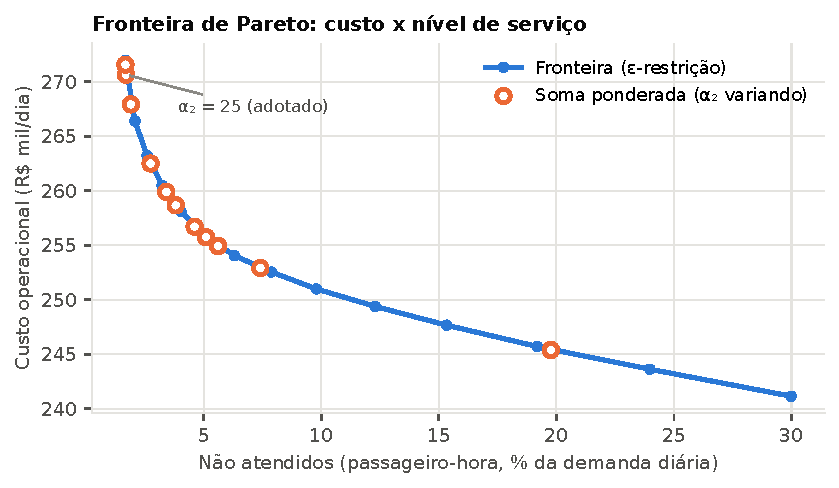
\includegraphics[width=0.85\textwidth]{fronteira_pareto.pdf}
\caption{Fronteira de Pareto custo operacional $\times$ espera excedente média.}
\label{fig:pareto}
\end{figure}

\begin{table}[htbp]
\centering
\caption{Soluções da soma ponderada para diferentes valores de $\alpha_2$.}
\label{tab:sensibilidade}
\small
\tabela{tabelas/sensibilidade.tex}
\end{table}

\subsection{Robustez}\label{sec:robustez}

A Tabela~\ref{tab:robustez} repete a instância calibrada com (i) um perfil
horário típico de corredor, independente da grade atual, e (ii) o modo
``perda''. Em ambos, o número de viagens e o custo variam pouco, o que indica
que as conclusões sobre a distribuição horária não dependem da circularidade do
perfil nem da hipótese sobre o comportamento do passageiro não atendido. O teste
não elimina, contudo, a dependência do rateio entre as linhas discutida acima.

\begin{table}[htbp]
\centering
\caption{Testes de robustez na instância calibrada.}
\label{tab:robustez}
\small
\tabela{tabelas/robustez.tex}
\end{table}

\subsection{Dualidade e pós-otimização}

O valor ótimo da relaxação linear é R\$~\Zrelax{} (gap de integralidade de
\gapInt\%). Pelo teorema das folgas complementares, o preço-sombra só é
positivo onde a restrição está ativa: na instância calibrada, apenas a frota
das \horaPrecoMax{} (R\$~\precoSombraMax{} por veículo; Tabela~\ref{tab:duais}).
As \faixasReotimizadas{} faixas foram re-otimizadas no PLIM com um veículo a
mais; houve ganho em \faixasGanhoPLIM{} delas. Às \horaPrecoMax{}, o ganho no
PLIM (R\$~\deltaPLIMMax{}) é menor que o preço-sombra porque o acréscimo de um
veículo ultrapassa o intervalo de validade do lado direito e porque as
frequências são inteiras. No limite inferior de demanda, todos os preços-sombra
da frota são nulos.

\begin{table}[htbp]
\centering
\caption{Restrições de frota e de corredor com valor marginal positivo, e validação no PLIM.}
\label{tab:duais}
\small
\tabela{tabelas/duais_frota.tex}
\end{table}

Os duais da restrição de atendimento~\eqref{eq:demanda} -- o custo marginal de
um passageiro a mais em $(l,t)$ -- se dividem, nos \nPares{} pares
linha-faixa, em: iguais ao custo por lugar $c/C$ quando a frota tem folga
(\regimeFolga{}); maiores que $c/C$ quando frota ou corredor estão no limite
(\regimeLimite{}); menores que $c/C$ quando o padrão de serviço já garante
capacidade de sobra (\regimeSobra{}); ligados a $\alpha_2$ quando há fila
(\regimeFila{}); e nulos nas faixas sem demanda (\regimeSemDemanda{}).

% =====================================================================
\section{Conclusões}\label{sec:conclusao}
% =====================================================================

Este trabalho formulou a definição de frequências e tipos de veículo das linhas
troncais do MOVE no Corredor Antônio Carlos como um PLIM com frota acumulada,
fila de passageiros, capacidade do corredor e padrão de serviço, resolvido de
forma exata pelo Gurobi em menos de um segundo.

Com a demanda calibrada pela grade atual, a solução ótima oferece mais serviço
que a grade programada por um custo \variacaoCusto\% maior, com a mesma frota.
O total de viagens de cada linha é determinado, em grande parte, pela forma como
os embarques das estações foram rateados entre as linhas; o valor agregado do
modelo está em decidir em que horas operar as viagens sob a restrição de frota.
A frota só se torna o gargalo do pico da manhã a partir de
$\lambda\approx\lambdaGargalo$; no limite inferior da demanda, ela sobra. Para
ampliar a oferta, articulados extras rendem mais por veículo que Padron, a
menos que o Padron seja sensivelmente mais barato por quilômetro e que seus
custos fixos sejam baixos.

Como trabalhos futuros, destacam-se: obter a carga medida no trecho crítico e a
demanda por linha nas estações (eliminando a dependência do rateio); incluir as
linhas alimentadoras e as transferências; incluir custos fixos de frota; e
estender o modelo ao projeto conjunto de linhas e frequências.

\afazer{Revisar as conclusões com a visão do grupo.}

\bibliographystyle{plainnat}
\bibliography{referencias}

\appendix
\section{Log do Gurobi (instância calibrada)}\label{ap:log}
{\footnotesize\verbatiminput{tabelas/log_gurobi_trecho.txt}}

\end{document}
